\documentclass[]{report}
\usepackage{amsmath}
\usepackage[spanish]{babel}
\usepackage[utf8]{inputenc}
\usepackage{graphicx}
\usepackage{booktabs}
\usepackage{float}
\usepackage[top=2cm, bottom=2cm, left=3cm, right=3cm]{geometry}

\title{Introducción al Modelado Continuo \\[0.5cm]
    Trabajo Práctico 3 \\[0.5cm]
    Resolución numérica de una ecuación de Poisson 1D}

\author{
    \textbf{Grupo: 11} \\[1cm]
    \begin{tabular}{lll}
        \textbf{Apellido} & \textbf{Nombre} & \textbf{Libreta} \\ \hline
        Wilders Azara & Santiago & 350/19 \\
        Peralta       & Martín   & 428/22 \\
        Vernay        & Jerónimo & 313/24 \\
    \end{tabular}
}

\date{\today}
\setlength{\parindent}{0pt}
\setlength{\parskip}{1ex plus .5ex minus .2ex}

\begin{document}
\maketitle

% ─────────────────────────────────────────────────────────────
\section*{Introducción}

Se busca resolver numéricamente la ecuación de Poisson en una dimensión, con una
condición de Dirichlet en $x=0$ y una de Neumann en $x=1$:
\begin{equation}
u''(x)=f(x),\quad x\in(0,1),\qquad u(0)=\alpha,\qquad u'(1)=\beta.
\label{eq:problema}
\end{equation}

Trabajamos sobre una malla uniforme $\{x_j=hj\}$, con $j=0,1,\dots,2^n+1$ y
$h=\dfrac{1}{2^n+1}$. Llamamos $M=2^n+1$ (de modo que $x_0=0$ y $x_M=1$) y tomamos
$n$ como parámetro de refinamiento. Como $u_0=\alpha$ es dato, las incógnitas son
$u_1,\dots,u_M$ y la matriz del sistema resulta de tamaño $M\times M$. La
Tabla~\ref{tab:malla} resume las mallas empleadas.

\begin{table}[H]
\centering
\begin{tabular}{rrl}
\toprule
$n$ & $M=2^n+1$ & $h=1/M$ \\
\midrule
3  & 9        & $1{,}11\times10^{-1}$ \\
4  & 17       & $5{,}88\times10^{-2}$ \\
5  & 33       & $3{,}03\times10^{-2}$ \\
6  & 65       & $1{,}54\times10^{-2}$ \\
7  & 129      & $7{,}75\times10^{-3}$ \\
8  & 257      & $3{,}89\times10^{-3}$ \\
9  & 513      & $1{,}95\times10^{-3}$ \\
10 & 1025     & $9{,}76\times10^{-4}$ \\
12 & 4097     & $2{,}44\times10^{-4}$ \\
14 & 16385    & $6{,}10\times10^{-5}$ \\
15 & 32769    & $3{,}05\times10^{-5}$ \\
23 & 8388609  & $1{,}19\times10^{-7}$ \\
\bottomrule
\end{tabular}
\caption{Mallas usadas: índice de refinamiento $k$, $n$, número de incógnitas $M$ y
	paso $h$. La instancia $k=3$ es el caso de inspección del Punto~1. Se observa también $k=3,\dots,14$ el barrido de
	error del Punto~2 y $k=22$ el mayor resuelto en el Punto~3.}
\label{tab:malla}
\end{table}

% ─────────────────────────────────────────────────────────────
\section*{Herramienta Matemática: Diferencias Finitas}

Se discretiza el dominio y se aproximan las derivadas del problema mediante desarrollos de Taylor. Para la derivada segunda en los nodos interiores, se emplea una diferencia centrada de orden 2:
\begin{equation}
u''(x_j)\approx\frac{u_{j-1}-2u_j+u_{j+1}}{h^2}.
\label{eq:centrada}
\end{equation}
Esta aproximación posee un error de truncamiento de orden $O(h^2)$ y es exacta para polinomios de grado menor o igual a 3. Por otra parte, para la condición de Neumann en el borde derecho ($x=1$), se utiliza una diferencia \textit{backward} de orden 2 a tres nodos:
\begin{equation}
u'(1)\approx\frac{3u_M-4u_{M-1}+u_{M-2}}{2h}=\beta.
\label{eq:backward}
\end{equation}
Esta expresión mantiene la consistencia con el esquema interior al presentar también un error de orden $O(h^2)$. Al ser ambas aproximaciones lineales respecto a los valores nodales, el problema se reduce a un sistema de ecuaciones lineales $Au=b$. Es importante notar que el número de condición de la matriz, $\kappa(A)$, crece proporcionalmente a $h^{-2}$, lo cual incrementará el impacto del error de redondeo a medida que se refine la malla.

\pagebreak

% ─────────────────────────────────────────────────────────────

\section*{Punto 1 -- Planteo del sistema $Au=b$}

Ordenamos las incógnitas como $u=(u_1,\dots,u_M)^\top$. Las filas interiores
($j=1,\dots,M-1$) usan \eqref{eq:centrada}; en la primera ($j=1$) el dato $u_0=\alpha$
pasa al lado derecho. La última fila ($j=M$) es la condición de Neumann
\eqref{eq:backward}. Resulta una matriz \textbf{casi tridiagonal}:
\begin{equation}
A=\begin{pmatrix}
-\frac{2}{h^2} & \frac{1}{h^2} & & & \\[2pt]
\frac{1}{h^2} & -\frac{2}{h^2} & \frac{1}{h^2} & & \\[2pt]
 & \ddots & \ddots & \ddots & \\[2pt]
 & & \frac{1}{h^2} & -\frac{2}{h^2} & \frac{1}{h^2}\\[2pt]
 & & \frac{1}{2h} & -\frac{4}{2h} & \frac{3}{2h}
\end{pmatrix},
\qquad
b=\begin{pmatrix}
\text{sen}(128\pi x_1)-\dfrac{\alpha}{h^2}\\[4pt]
\text{sen}(128\pi x_2)\\
\vdots\\
\text{sen}(128\pi x_{M-1})\\[2pt]
\beta
\end{pmatrix}.
\label{eq:sistema}
\end{equation}

\textbf{Observación sobre la matriz $A$:} La matriz resultante no es simétrica, dado que la fila correspondiente a la condición de Neumann está escalada por un factor de $1/(2h)$ en lugar de $1/h^2$.

\textbf{Verificación ($n=3$):} Para este nivel de refinamiento, se tiene $M=2^3+1=9$ incógnitas ($h=1/9\approx0{,}1111$, de modo que $1/h^2=81$ y $1/(2h)=4{,}5$). La matriz $A$ presenta una diagonal principal de valor $-162$, codiagonales de $81$ y una última fila con los coeficientes $(4{,}5,\,-18,\,13{,}5)$. El error en norma infinito obtenido es de aproximadamente $0{,}19$, un valor significativo en comparación con la norma de la solución analítica. Este error se debe a que la función seno de alta frecuencia ($128\pi$) se encuentra insuficientemente muestreada con $9$ nodos, fenómeno que se analiza en detalle a continuación.

% ─────────────────────────────────────────────────────────────
\section*{Punto 2 -- Error y orden del método}

Para $f(x)=\text{sen}(128\pi x)$, integrando dos veces e imponiendo las condiciones de contorno $\alpha=2$, $\beta=1$, la solución exacta es
\begin{equation}
u(x) = -\frac{1}{(128\pi)^2} \text{sen}(128\pi x) + \left(1 + \frac{1}{128\pi}\right)x + 2 .
\end{equation}

Resolvemos el sistema \eqref{eq:sistema} para $n=3,\dots,14$ y medimos el error en norma infinito en función de $h$ (Figura~\ref{fig:item2}).

\textbf{Interpretación Numérica: Aliasing y Teorema de Nyquist.} La función fuente seleccionada presenta 64 oscilaciones completas en el intervalo $[0,1]$. De acuerdo con el teorema de muestreo de Nyquist, es necesario disponer de al menos dos nodos por período para evitar el fenómeno de \textit{aliasing}. En este caso particular, se requiere un mínimo de $M > 128$ nodos (correspondiente a $n \ge 7$) para capturar adecuadamente la señal.

Como ilustra la Figura~\ref{fig:item2_perfil}, para $n=6$ ($M=65$ nodos) la malla carece de la resolución necesaria, resultando en un muestreo insuficiente que impide al esquema numérico aproximar la solución oscilatoria de forma correcta. Esto se refleja en la fase inicial del gráfico de convergencia (Figura~\ref{fig:item2}), donde para $n<7$ el error se mantiene elevado y sin un patrón de descenso estable. Una vez superado el límite impuesto por el teorema de Nyquist, la frecuencia es capturada correctamente, como se aprecia en el perfil para $n=9$ ($M=513$). A partir de allí se observa la fase asintótica, donde se evidencia la convergencia teórica de orden 2 propia del método: ajustando la pendiente del gráfico log-log en la rama convergente ($n=9,\dots,14$) se obtiene un valor de $\approx1{,}97$, consistente con el orden $O(h^2)$ dominado por el error de truncamiento.

\begin{figure}[H]
\centering

\includegraphics[width=0.6\linewidth]{../figuras/item2_error_vs_h.png}
\caption{Error en norma infinito vs $h$ para $f=\text{sen}(128\pi x)$. Orden 2 (pendiente $\approx1{,}97$) visible una vez superado el aliasing de la alta frecuencia.}
\label{fig:item2}
\end{figure}

\begin{figure}[H]
\centering
\begin{minipage}{0.49\textwidth}\centering
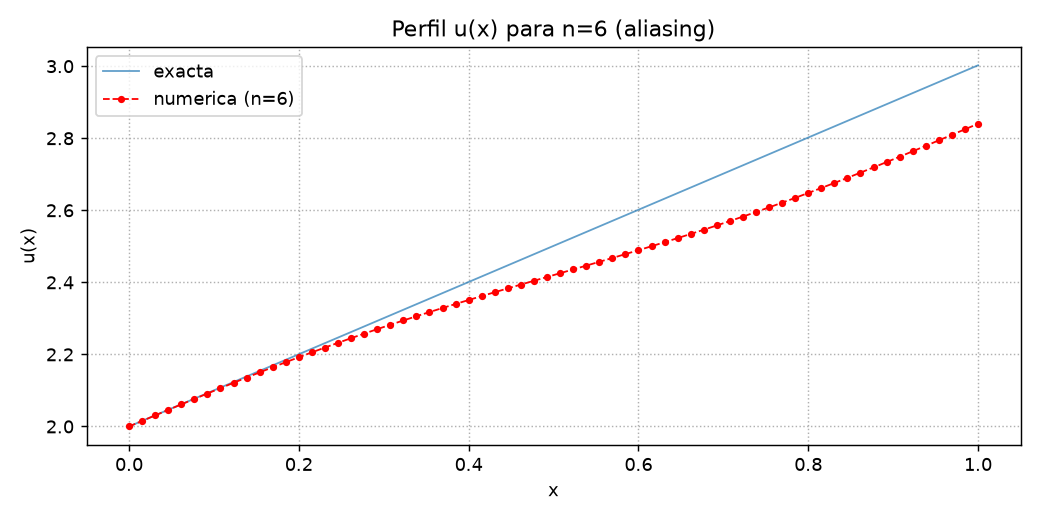
\includegraphics[width=\linewidth]{../figuras/item2_perfil_n6.png}
\caption{Perfil de $u(x)$ para $n=6$ ($M=65$): submuestreo severo y fallo por aliasing.}
\label{fig:item2_perfil}
\end{minipage}\hfill
\begin{minipage}{0.49\textwidth}\centering
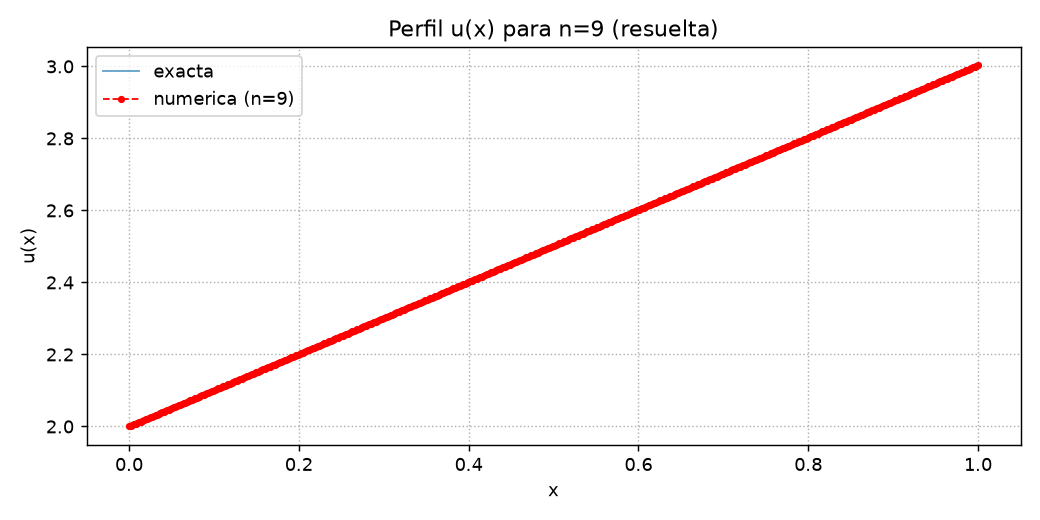
\includegraphics[width=\linewidth]{../figuras/item2_perfil_n9.png}
\caption{Perfil de $u(x)$ para $n=9$ ($M=513$): la onda queda bien resuelta.}
\label{fig:item2_perfil_n9}
\end{minipage}
\end{figure}

% ─────────────────────────────────────────────────────────────
\section*{Punto 3 -- $f(x)=e^{-x^2}$ con matrices esparsas}

Repetimos el planteo del Punto~1 para $f(x)=e^{-x^2}$, $\alpha=2$, $\beta=1$, ahora
ensamblando $A$ como matriz esparsa (\texttt{scipy.sparse}) y resolviendo con
\texttt{spsolve}. La solución exacta se obtiene integrando, usando
$\int e^{-x^2}\,dx=\tfrac{\sqrt\pi}{2}\operatorname{erf}(x)$:
\begin{equation}
u'(x)=\beta-\tfrac{\sqrt\pi}{2}\operatorname{erf}(1)+\tfrac{\sqrt\pi}{2}\operatorname{erf}(x),
\qquad
u(x)=\alpha+\int_0^x u'(s)\,ds ,
\end{equation}
que se evalúa con \texttt{scipy.special.erf}. La Figura~\ref{fig:item3perfil} compara el
perfil numérico con el exacto.

Al ser un caso no polinómico (y sin problemas de Nyquist), la convergencia de orden 2 se observa inmediatamente: ajustando la pendiente en la rama convergente ($n=3,\dots,15$) se obtiene $\approx+2{,}03$ (Figura~\ref{fig:item3}). A partir de $n\approx15$ el error deja de bajar y empeora debido a la amplificación del redondeo ($\kappa(A) \sim h^{-2}$).

\begin{figure}[H]
\centering
\begin{minipage}{0.49\textwidth}\centering

\includegraphics[width=\linewidth]{../figuras/item3_error_vs_h.png}
\caption{Orden 2 en la convergencia y subida por redondeo.}
\label{fig:item3}
\end{minipage}\hfill
\begin{minipage}{0.49\textwidth}\centering

\includegraphics[width=\linewidth]{../figuras/item3_perfil.png}
\caption{Perfil $u(x)$ para $n=23$ (submuestreado para graficar).}
\label{fig:item3perfil}
\end{minipage}
\end{figure}

\textbf{Límites Computacionales:} En la evaluación sobre una máquina local se logró resolver el sistema hasta $\mathbf{n=23}$, lo que equivale a $M\approx8{,}4\times10^6$ incógnitas. Al intentar refinar a $n=24$ ($M\approx16{,}8\times10^6$), el procedimiento se interrumpe por falta de memoria durante la ejecución del solver (\texttt{spsolve}).

El factor limitante \textbf{no} es el almacenamiento de la matriz $A$ (esparsa, $O(M)$) ni el \emph{fill-in} de la factorización. De hecho, al ser $A$ casi tridiagonal, el factor LU casi no se llena: medimos $\operatorname{nnz}(L)+\operatorname{nnz}(U)\approx1{,}33\cdot\operatorname{nnz}(A)$, una razón que se mantiene constante al refinar la malla. La restricción real es la \emph{memoria total} que \texttt{spsolve}/SuperLU necesita para construir y almacenar la factorización LU junto con sus estructuras internas de control: crece como $O(M)$ pero con una constante grande y, en torno a $M\approx16{,}8$ millones, agota la RAM de la máquina. Por otra parte, el límite de \emph{utilidad numérica} se alcanza mucho antes, en $n\approx15$: refinamientos posteriores no mejoran la exactitud porque la amplificación del error de redondeo de punto flotante ($\kappa(A)\sim h^{-2}$) comienza a dominar sobre la reducción del error de truncamiento.

% ─────────────────────────────────────────────────────────────
\section*{Conclusiones}

\begin{itemize}
  \item El esquema de diferencias finitas centrado acoplado con backward de orden 2 en la frontera es consistente y convergente de \textbf{orden 2} (pendientes medidas $\approx1{,}97$ y $\approx2{,}03$).
  \item Problemas con soluciones de altísima frecuencia (como $\text{sen}(128\pi x)$) requieren mallas muy finas no solo para alcanzar una tolerancia estricta, sino para apenas evadir los problemas graves de aliasing y representatividad cualitativa de la onda.
  \item Las matrices esparsas permiten escalar hasta mallas masivas ($n=23$, $\approx 8{,}4$ millones de grados de libertad), pero el límite lo fija la \emph{memoria} que requiere la factorización LU dentro de \texttt{spsolve} (no el fill-in, que es despreciable), y la ganancia de precisión se estanca en el piso de redondeo inherente a la aritmética de punto flotante en torno a $n\approx15$.
\end{itemize}

\end{document}
